\begin{frame}
  \frametitle{Freie Software auf Computern}
    \begin{columns}
        \begin{column}{5cm}
            \begin{center}
                
\includegraphics[height=0.2\textheight]{img/firefox.png} \\
                Firefox \\
                \vspace{0.1\textheight}
                
\includegraphics[height=0.2\textheight]{img/libreoffice.jpg}\\
                LibreOffice
            \end{center}
        \end{column}
        \begin{column}{5cm}
            \begin{center}
                
\includegraphics[height=0.2\textheight]{img/thunderbird.png} \\
                Thunderbird \\
                \vspace{0.1\textheight}
                
\includegraphics[height=0.2\textheight]{img/vlc.png}\\
                VLC Media Player
            \end{center}
        \end{column}
    \end{columns}
\end{frame}

\note{Open Source Software oder Freie Software gibt es in allen Bereichen. Oft verwenden wir sogar freie Programme ohne es zu wissen. Auf der Folie sind 4 bekannte Beispiele aufgeführt}

\begin{frame}{Freie Software auf dem Smartphone}
  \begin{columns}
    \column{6.5cm}

    \textbf{F-Droid}\\
    Android-Appstore für freie Software

    \vspace{0.5cm}

    \textbf{iOS Open Source Apps}\\
    \url{https://github.com/dkhamsing/open-source-ios-apps}

    \column{5cm}

    \begin{center}
      
\includegraphics[width=2cm]{img/F-Droid_Logo_2}
    \par\end{center}
    \begin{center}
    \par\end{center}
  \end{columns}
\end{frame}

\note{Auf dem Smartphone ist es etwas komplizierter, freie Apps zu finden und zu installieren. Auf Android gibt es viele open source Apps im Google Play Store, diese sind jedoch selten als solche zu erkennen. Einfacher ist die Nutzung von F-Droid, einem alternativen App-Store für Android, der ausschließlich Open Source Software beinhaltet. F-Droid bietet viele interessante Eigenschaften, beispielsweise informiert es darüber, ob Apps Daten versenden und wenn ja an wen. Unter iOS gibt es eine eher kurze Auflistung an Open Source Apps im AppStore. Das bekannteste Beispiel ist der Signal messenger, der später nochmal aufgegriffen wird.}

\begin{frame}{F-Droid}
  \begin{columns}
    \column{6.5cm}

    \begin{center}
      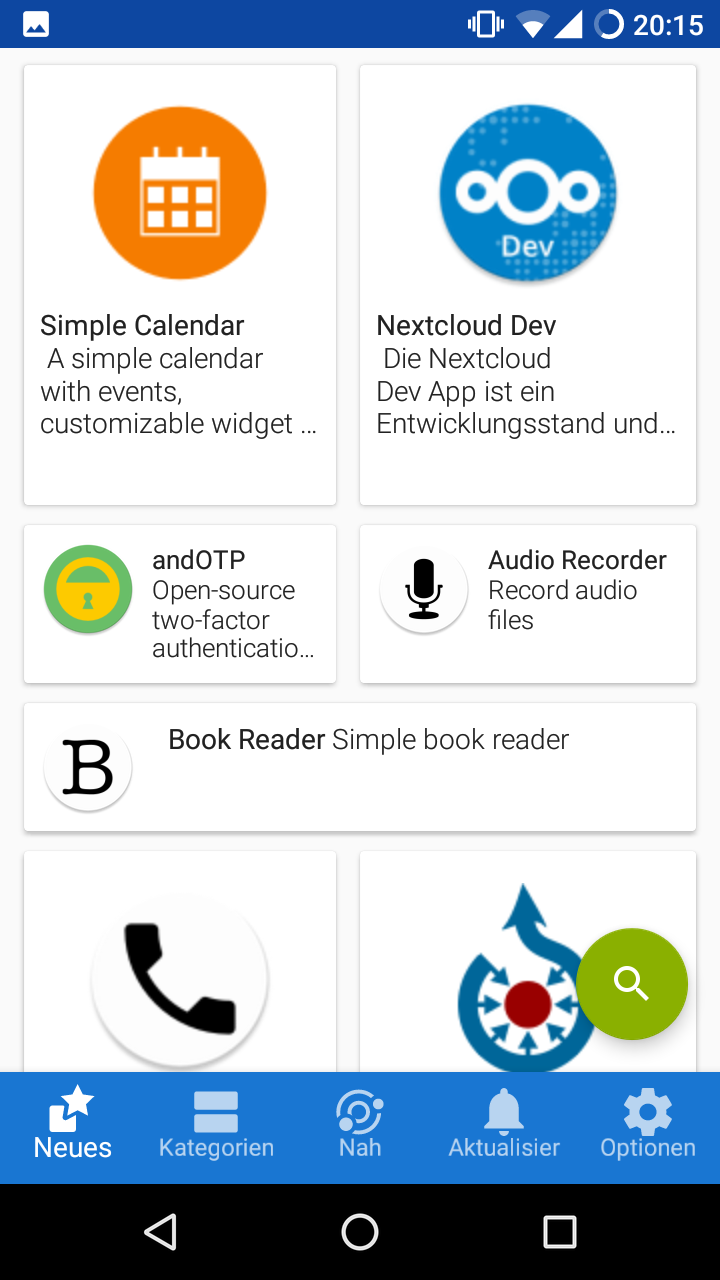
\includegraphics[height=6cm]{img/fdroid1.png}
    \par\end{center}

    \column{5cm}

    \begin{center}
      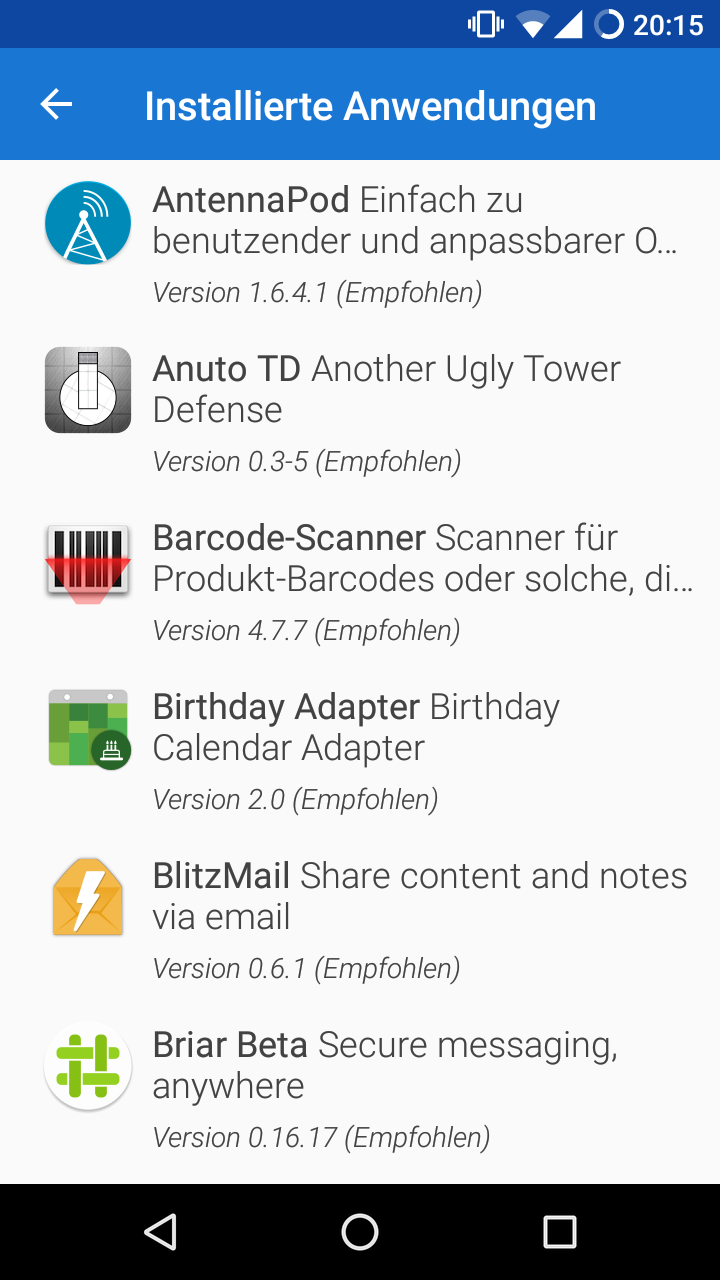
\includegraphics[height=6cm]{img/fdroid2.png}
    \par\end{center}
  \end{columns}
\end{frame}
